\section{The Database: NeuroMorphic15}
\label{sec:data}
\subsection{Current Status}
what are the problems the current database aim for.
Current methods/algorithms existing.


The FERET tests are administered using a testing proto-
col, which states the mechanics of the tests and the manner
in which the test will be scored. In face recognition, for
example, the protocol states the number of images of each
person in the test, how the output from the algorithm is
recorded, and how the performance results are reported.
There is a direct connection among the problem being
evaluated, the images in the database, and the testing pro-
tocol. The testing protocol and the images define the pro-
blem to be evaluated. The characteristics and quality of the
images are major factors in determining the difficulty of the
problem. For example, if the faces are in a predetermined
position in the images, the problem is different from that for
images in which the faces can be located anywhere in the
image. In the FERET database, variability was introduced
by the inclusion of images taken at different dates and loca-
tions (see Section 4.2). This resulted in changes in lighting,
scale, and background.
The goals for the FERET evaluation process were to assess
the state of the art, advance the state of the art, and point to
future directions of research. Accomplishing all three goals
was a delicate process, and the keys to success were the
database and the tests. If algorithms existed that could easily
solve the problem, then the evaluation process would be
reduced to ‘tuning’ existing algorithms. On the other hand,
if the images defined a problem that was beyond current
algorithmic techniques, then the results would have been
poor and would have not allowed an accurate assessment of
current algorithmic capabilities. The key was to find the right
balance, so that if the problem formulated could not be solved
satisfactorily by existing methods, it would be possible to
develop algorithms that could solve it.
The collection of the FERET database was initiated in
September 1993, and the first FERET test was administered
in August 1994. A standard database of facial images was
established in the first year and made available to research-
ers; this database provided the images for the Aug94
FERET test. (Throughout this article, date-based names
such as Aug94 are used to refer to the same FERET test,
even when the tests were administered on other dates.) The
Aug94 FERET test established a performance baseline for
fully automatic face-recognition
algorithms. A fully auto-
matic algorithm does not require the location of the face in
the image as input: the algorithm locates and identifies the
face in the image.
The Aug94 FERET test was designed to measure the
performance of algorithms that could automatically locate,
normalize, and identify faces from a database. The test
consisted of three subsets: the large gallery, false alarm,
and rotation tests. The first tested the ability of algorithms
to recognize faces from a set of 317 known individuals
(referred to as the gallery; an image of an unknown face
presented to the algorithm is a probe, and the collection of
probes is called the probe set). The second subtest, the false-
alarm test, measured how well an algorithm rejects faces not
in the gallery. The third baselined the effects of pose
changes (rotations) on performance. On the basis of the
Aug94 FERET test, it was concluded that algorithms needed
to be evaluated on (1) larger galleries and (2) a substantially
increased number of duplicate probes. (A duplicate is
defined as an image of a person whose corresponding
gallery image was taken on a different date.)
A second FERET test, first administered in March 1995
(and referred to as the Mar95 FERET test), was designed
based on the conclusions from the Aug94 FERET test. The
Mar95 FERET test evaluated algorithms on larger galleries
and probe sets with a greater number of duplicates. This
required that additional images be collected, with an emphasis
on images of the same people taken months or years apart.

\subsubsection{Converting from MPL to SNN}
It remains a challenge to transform traditional artificial neural networks into spiking ones.
There are attempts~\cite{la2008response}~\cite{burkitt2006review} to estimate the output firing rate of the LIF neurons (Equation~\ref{equ:lif}) under certain conditions. 
%For the model illustrated above, there are two types of synaptic connection: one-to-one connections in the retina layer and N-to-one connections in all the convolutional layers (the pooling layer is also included). 
%For the retina layer, 1) the problem is: what is the connection weight between two single LIF neurons to make a post-synaptic neuron fire whenever the pre-synaptic neuron generates a spike? 
%While for the convolutional neurons, 2) given the input spike rates, LIF neuron parameters and the output spiking rate, what are the corresponding weights between the two layers?
\begin{equation}
\frac{\D \: V(t)}{\D\:  t}=-\frac{V(t)-V_\mathit{rest}}{\tau_m}+\frac{I(t)}{C_m}
\label{equ:lif}
\end{equation}
The membrane potential $V$ changes in response to input current $I$, starting at the resting membrane potential  $V_{rest}$, where the membrane time constant is $\tau_m = R_mC_m$, $R_m$ is the membrane resistance and $C_m$ is the membrane capacitance.

Given a constant current injection $I$, the response function, i.e. firing rate, of the LIF neuron is
\begin{equation}
\lambda_\mathit{out}=
\left [ t_\mathit{ref}-\tau_m\ln \left ( 1-\frac{V_{th}-V_\mathit{rest}}{IR_m}  \right )\right ]^{-1}
\label{equ:consI}
\end{equation}
when $IR_m>V_{th}-V_{rest}$, otherwise the membrane potential cannot reach the threshold $V_{th}$ and the output firing rate is zero. 
The absolute refractory period $t_\mathit{ref}$ is included, where all input during this period is invalid.
In a more realistic scenario, the post-synaptic potentials (PSPs) are triggered by the spikes generated from the neuron's pre-synaptic neurons other than a constant current.
Assume that the synaptic inputs are Poisson spike trains, the membrane potential of the LIF neuron is considered as a diffusion process. Equation~\ref{equ:lif} can be modelled as a stochastic differential equation referring to Ornstein-Uhlenbeck process,
\begin{equation}
\tau_m\frac{\D\:V(t)}{\D\:  t}=-\left[V(t)-V_\mathit{rest}\right] + \mu + \sigma\sqrt{2\tau_m}\xi (t)
\label{equ:sde}
\end{equation}
where
\begin{equation}
\begin{array}{l}
\mu=\tau_m(\mathbf{w_E\cdot\lambda_E}-\mathbf{w_I\cdot\lambda_I})
\\
\\
\sigma ^{2} = \frac{\tau_m}{2}\left(\mathbf{w_E^{2}\cdot\lambda_E}+\mathbf{w_I^{2}\cdot\lambda_I}\right)
\end{array}
\label{equ:ou}
\end{equation}
are the conditional mean and variance of the membrane potential.
The delta-correlated process $\xi(t)$ is Gaussian white noise with zero mean, $\mathbf{w_E}$ and $\mathbf{w_I}$ stand for the weight vectors of the excitatory and the inhibitory synapses, and $\mathbf{\lambda}$ represents the vector of the input firing rate.
The response function of the LIF neuron with Poisson input spike trains is given by the Siegert function~\cite{siegert1951first}, 
%\begin{equation}
%%\lambda_\mathit{out}=\left(\tau_\mathit{ref} + \frac{\tau_Q}{\sigma_Q}\sqrt{\frac{\pi}{2}} \int_{V_\mathit{rest}}^{V_\mathit{th}}du \:\exp \left(\frac{u-\mu_Q}{\sqrt2\sigma_Q} \right )^{2}\left[1+erf \left(\frac{u-\mu_Q}{\sqrt2\sigma_Q} \right ) \right ]\right)^{-1}
%\begin{split}
%\lambda_\mathit{out}=\left(\tau_\mathit{ref} + \frac{\tau_Q}{\sigma_Q}\sqrt{\frac{\pi}{2}} \int_{V_\mathit{rest}}^{V_\mathit{th}}\D u \:\exp \left(\frac{u-\mu_Q}{\sqrt2\sigma_Q} \right )^{2}\left[1+\mathrm{erf} \left(\frac{u-\mu_Q}{\sqrt2\sigma_Q} \right ) \right ]\right)^{-1}
%\end{split}
%\label{equ:sgt}
%\end{equation}
\begin{align}
\lambda_\mathit{out} &=\left(\tau_\mathit{ref} + \frac{\tau_Q}{\sigma_Q}\sqrt{\frac{\pi}{2}} \int_{V_\mathit{rest}}^{V_\mathit{th}}\D\,u \:\exp \left(\frac{u-\mu_Q}{\sqrt2\sigma_Q} \right )^{2} \right. \nonumber \\
&\qquad \left. \vphantom{\int_t} \cdot  \left[1+\mathrm{erf} \left(\frac{u-\mu_Q}{\sqrt2\sigma_Q} \right ) \right ]\right)^{-1}
\label{equ:sgt}
\end{align}
where $\tau_Q, \mu_Q, \sigma_Q$ are identical to $\tau_m, \mu, \sigma$ in Equation~\ref{equ:ou}, and erf is the error function.

Still there are some limitations on the response function. 
For the diffusion process, only small amplitude (weight) of the PostSynaptic Potentials (PSPs) generated by a large amount of input spikes (high spiking rate) work under this circumstance; 
plus, the delta function is required, i.e. the synaptic time constant is considered to be zero. Thus only a rough approximation of the output spike rate has been determined.
Secondly, given different input spike rate to each pre-synaptic neurons, the parameters of the LIF neuron and the output spiking rate, how to tune every single corresponding synaptic weight remains a difficult task.

\subsubsection{Rank-Order-Coding}

\subsubsection{Liquid State Machine/Reservoir Encoding}

\subsection{Description}
	Experiment setup/ collection method/ properties of each class/ etc.
	\subsubsection{Poisson}
	\subsubsection{Rank-Order-Encoding}
  A different way of encoding spikes is using a \emph{rank-order}; this means
keep just the order in which those spikes were fired and disregard the exact timing. One can think of this as a compromise between the complexity of time-based encoding and the small capacity to represent information of rate-based codes. Rank-ordered spike trains have been used in vision tasks under a biological plausibility constraint, making them a viable way of image encoding for neural applications~[\cite{van-rullen-rate-coding,basab-model}].

We perform rank-ordered encoding using an algorithm known as 
\emph{FoCal}~[\cite{basab-model}]. It models the \emph{foveal pit} region, the highest resolution area of the retina. As a first step four discrete 2D \emph{convolutions} are performed. Each convolution simulates a ganglion cell type and every cell is modelled using Differences of Gaussians (DoG, Eq.~\ref{eq-dog}). 
\begin{equation}
\label{eq-dog}
DoG_w(x,y) = \pm\frac{1}{2\pi\sigma_{w,c}^2}e^{\frac{-(x^2 + y^2)}{2\sigma_{w,c}^2}}
\mp\frac{1}{2\pi\sigma_{w,s}^2}e^{\frac{-(x^2 + y^2)}{2\sigma_{w,s}^2}}
\end{equation}
where $\sigma_{w,c}$ and $\sigma_{w,s}$ are the standard deviation for the 
centre and surround components of the DoG at scale $w$ (cell type). The signs 
will be ($-$,$+$) if the ganglion cell has an \emph{off-centre} behaviour and 
($+$,$-$) if it has an \emph{on-centre} one. Table~\ref{tab-kernel-specs} 
describes the parameters used to compute the convolution \emph{kernels} at each 
scale $w$.

\begin{table}[htb]
  \caption{Simulation parameters for ganglion cells}
  \centering
  \begin{tabular}{l c c c c}
    \begin{minipage}{1.2cm}Cell type \end{minipage}& 
    \begin{minipage}{1cm} \centering Matrix width \end{minipage}&  
    \begin{minipage}{1.3cm}\centering Centre std. dev. ($\sigma_c$)\vspace*{0.1cm}\end{minipage} & 
    \begin{minipage}{1.3cm}\centering Surround std. dev. ($\sigma_s$)\vspace*{0.1cm}\end{minipage} & 
    \begin{minipage}{1.3cm}\centering Sampling resolution (cols,rows)\vspace*{0.1cm}\end{minipage} \\
    \hline
    \begin{minipage}{1.32cm}\vspace*{0.1cm} Midget Off-centre \vspace*{0.005cm} \end{minipage}& 
    \begin{minipage}{1cm}\centering$3$ \end{minipage}& 
    $0.8$ & $6.7 \times \sigma_c$ &  1, 1 \\
    \begin{minipage}{1.32cm} Midget On-centre \vspace*{0.005cm}\end{minipage} & 
    \begin{minipage}{1cm}\centering $11$ \end{minipage}& 
    $1.04$ & $6.7 \times \sigma_c$ & 1, 1 \\
    \begin{minipage}{1.32cm}Parasol Off-centre \vspace*{0.005cm}\end{minipage} & 
    \begin{minipage}{1cm}\centering $61$ \end{minipage}& 
    $8$ & $4.8 \times \sigma_c$ & 5, 3 \\
    \begin{minipage}{1.32cm} Parasol On-centre \vspace*{0.005cm}\end{minipage} & 
    \begin{minipage}{1cm}\centering $243$\end{minipage} &
    $10.4$ & $4.8 \times \sigma_c$ & 5, 3 
  \end{tabular}
  \label{tab-kernel-specs}
\end{table}

Every pixel value in the convolved images (Fig. \ref{fig-convolution-results}) 
is inversely proportional to a spike emission time (i.e. the higher the pixel value, the sooner the spike will be sent out.)

\begin{figure}[hbt]
  \centering
  \subfloat[Original image]{
    \label{sfig-rank-ordered-original}
    
\includegraphics[width=0.15\textwidth]{original_5_1}
  }
  \subfloat[Midget Off-centre]{
    \label{sfig-rank-ordered-midget-off}
    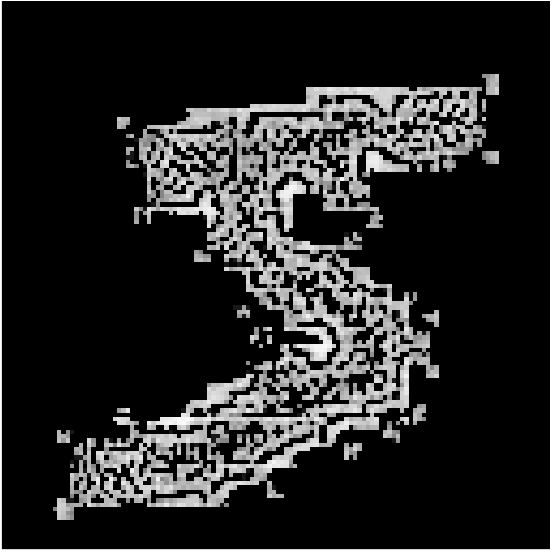
\includegraphics[width=0.15\textwidth]{filtered_focal_5_1_0}
  }
  \subfloat[Midget On-centre]{
    \label{sfig-rank-ordered-midget-on}
    
\includegraphics[width=0.15\textwidth]{filtered_focal_5_1_1}
  }\\
  \subfloat[Parasol Off-centre]{
    \label{pic-lena-P-OFF}
    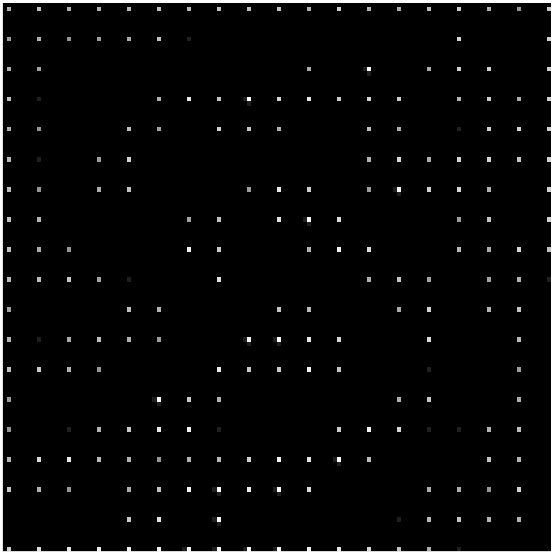
\includegraphics[width=0.15\textwidth]{filtered_focal_5_1_2}
  }
  \subfloat[Parasol On-centre]{
    \label{pic-lena-P-ON}
    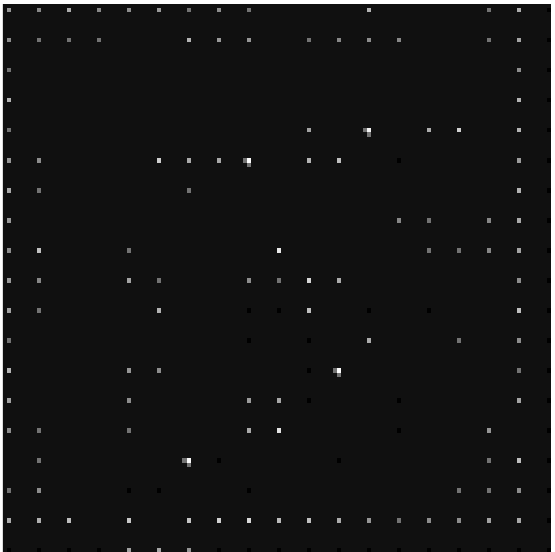
\includegraphics[width=0.15\textwidth]{filtered_focal_5_1_3}
  }
  \caption{Results of simulating ganglion cells (convolved images are enhanced for better contrast)}
  \label{fig-convolution-results}
\end{figure}
The algorithm also performs redundancy a correction step; it does so by 
adjusting the convolved image's pixel value according to the correlation 
between convolution kernels. At each iteration of the correction step, the 
maximum coefficient value of \emph{all images} is selected, ``taken out'' and its 
surrounding pixels get adjusted (Alg.~\ref{code-focal-corr}).
\begin{algorithm}[h]
  \caption{FoCal, Part 2}
  \label{code-focal-corr}
  \begin{algorithmic}
    \Procedure{Correction}{coeffs $C$, correlations $Q$}
    \State $N \leftarrow \emptyset$ \Comment{Corrected coefficients}
    \Repeat
    \State $m \leftarrow max(C)$\Comment{Obtain maximum from $C$}
    \State $M \leftarrow M \cup m$\Comment{Add maximum to $M$}
    \State $C \leftarrow C \setminus m$\Comment{Remove maximum from $C$}
    \ForAll{$ c \in C$} \Comment{Adjust all remaining $c$}
    \If{$Q(m, c) \neq 0$} \Comment{Adjust only near}
    \State $c \leftarrow c - m \times Q(m, c)$
    \EndIf
    \EndFor
    \Until{$C = \emptyset$}
    \State \textbf{return} $M$
    \EndProcedure
  \end{algorithmic}
\end{algorithm}
Two resolutions are provided for the rank-order encoded database, the first is 
the original $28\times28$ one. An additional up-scaled resolution version is also provided, the images where scaled to a $128\times128$ resolution using bi-cubic interpolation, this was done to match the DVS native resolution. The format of the data is not exactly AER since keeping spiking order is what matters for this encoding; depending
on the experimenter's needs the timing between spikes can be modified. The adjusted weights and cell origin have been preserved for further processing.
	\subsubsection{DVS Sensor Output with Flashing Input}
	\subsubsection{DVS Sensor Output with Oscillating Input}
	\subsubsection{DVS Sensor Output with Moving Input}
	